En toda la sección de experimentación vamos a analizar las distintas métricas usualmente observadas en los sistemas de categorización. Principalmente exactitud (accuracy), precisión, recall y f1, para más explicación de cada una de ellas pueden referirse a \cite{metricasPaper} o más visualmente en \cite{metricasWeb}

\documentclass[a4paper,10pt]{article}
\usepackage[utf8]{inputenc}
\usepackage{graphicx}
\usepackage{float}
\usepackage{hyperref}
\usepackage{caption}
\usepackage{subcaption}


%opening
\title{}
\author{}

\begin{document}

\section{Búsqueda de parámetros óptimos }

El principal objetivo de esta sección es encontrar los parámetros óptimos de knn y knn+pca con respecto a la accuracy. 

\subsection{Experimentación preliminar}
Este primer segmento de la sección se enfoca en generar una intuición sobre cómo reaccionan los métodos frente a distintos valores de k, alpha para ello utilizamos una partición del dataset original para poder experimentar sobre un rango bastante extenso de parámetros sin preocuparnos demásiado por la complejidad. Este primer experimento consiste en utilizar un split simple de train y validación sobre la partición previamente elegida para cada k en el caso de kNN y para cada pareja alpha, k en caso de kNN+PCA. 

\subsubsection{kNN}

\begin{figure}[h]
\begin{subfigure}{0.5\textwidth}
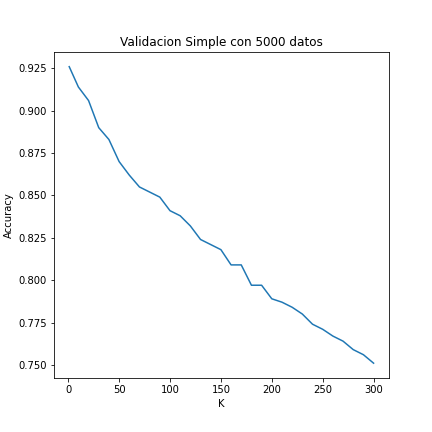
\includegraphics[width=0.9\linewidth, height=5cm]{../images/validacionSimple_knnsolo.png} 
\caption{Rango de 1-300 con granularidad 10}
\label{fig:subimbar_medio1}
\end{subfigure}
\begin{subfigure}{0.5\textwidth}
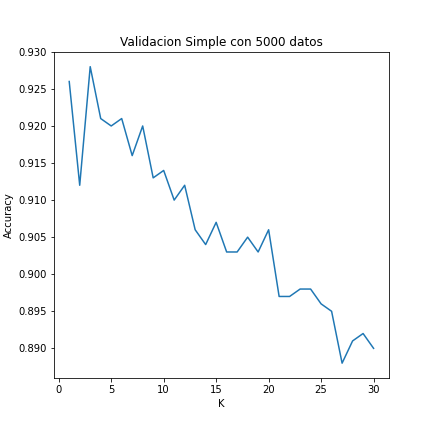
\includegraphics[width=0.9\linewidth, height=5cm]{../images/validacionSimple_knnsolo_Kchicos.png} 
\caption{Rango de 1-30 con granularidad 1}
\label{fig:subimbar_medio2}
\end{subfigure}
\caption{Validacion Simple de kNN sobre el data-set reducido.}
\label{knn_preliminar}%
\end{figure}

\par

Como podemos primer en la imagen (a) de Figura 1 muestra una presunta relación inversamente proporcional entre el k elegido y su accuracy, para vislumbrar si esto es así realizamos el mismo experimento sobre valores pequeños de k pero con más granularidad para notar cualquier variación en la accuracy, que es lo que se puede observar en la imagen (b). Ahora con más detalle se puede observar a partir de cuales magnitudes el método disminuye se eficiencia, en particular los mejores k parecen encontrarse dentro del rango 1-10.

\subsubsection{kNN+PCA}

\begin{figure}[H]
    \centering
    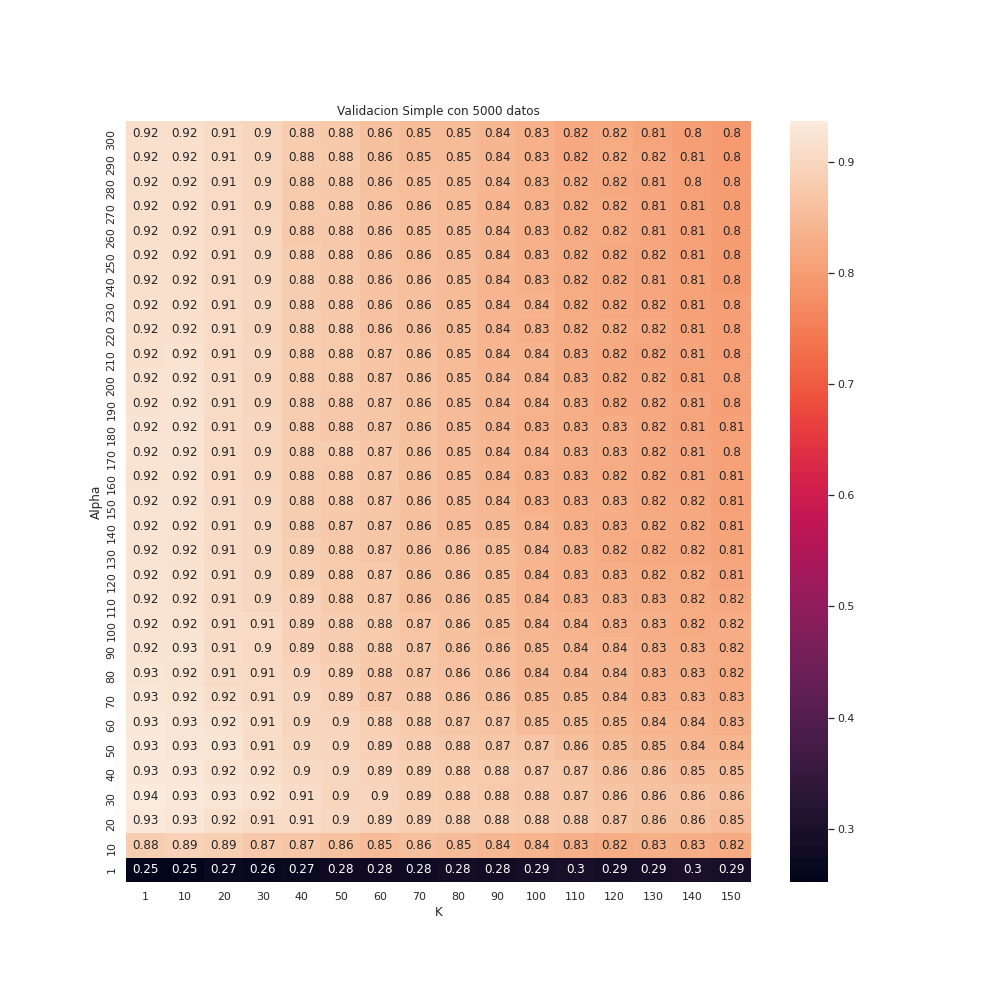
\includegraphics[width=12cm]{../images/validacionSimple_heatmap_datasetRedux}%
    \qquad
    \caption{Validacion Simple de kNN+PCA sobre el data-set reducido}
    \label{knnpca_preliminar}%
\end{figure}

Al igual que sucede en kNN podemos notar un mejor desempeño para las parejas con valores chicos de $k$, en cambio para alpha ya no estan clara la relación aunque se puede ver una leve mejora para los $alpha$ menores a 100, por esto mismo en la validacion simple que sigue sobre el dataset en su totalidad mantendremos el rango del $alpha$ y solo achicaremos el de $k$.

\subsection{Validación Simple sobre el data-set completo}

La segunda parte de esta sección realiza el mismo experimento que la primera pero ahora sobre el dataset original y eligiendo un rango condicionado por lo antes visto, con la motivación de encontrar el conjunto de los mejores diez parámetros para cada método. Notese que cuando decimos que el rango del experimento estara condicionado por una experimentacion realizada sobre un dataset reducido ,estamos asumiendo que los parámetros se ven inmutables por la cantidad de datos para entrenar y validar lo cual no es trivial por esa razon lo analizamos en la SECCION FER, donde mostramos empiricamente que esto es verdadero para nuestro caso particular.


\subsubsection{kNN}


\begin{figure}[H]
    \centering
    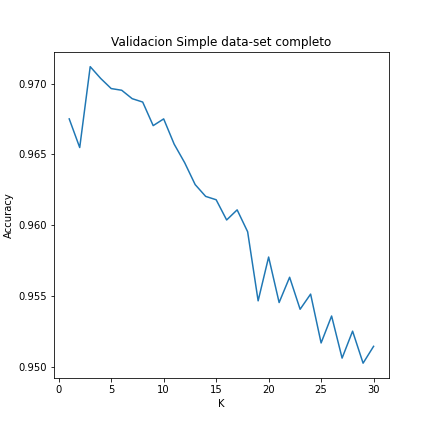
\includegraphics[width=8cm]{../images/validacionSimple_datasetCompleto.png}%
    \qquad
    \caption{Validacion Simple de kNN sobre el data-set completo}
    \label{knn_valSimple}%
\end{figure}

\begin{table}[h!]
    \begin{center}
        \begin{tabular}{|c|c|}
        \hline
        \textbf{$k$} & \textbf{accuracy} \\
        \hline
        3 &  0.9711\\
        4 & 0.9703\\
        5 & 0.9696\\
        6 & 0.9695\\
        7 &  0.9689\\
        8 & 0.9686\\
        1 & 0.9675\\
        10 & 0.9675\\
        9 & 0.9670\\
        11 & 0.9657\\
        
        \hline
        \end{tabular}
        \caption{Accuracy de las mejores 10 parejas extraido de la Validacion Simple sobre el dataset completo para kNN.}
        \label{knn_valSimple_table}
    \end{center}
\end{table}

\subsubsection{kNN+PCA}

\par

$ k \in \{1,..,80\}$ (granularidad = 2)\\$alpha \in \{  35, 160 \}$ (granularidad = 5)

\begin{figure}[H]
    \centering
    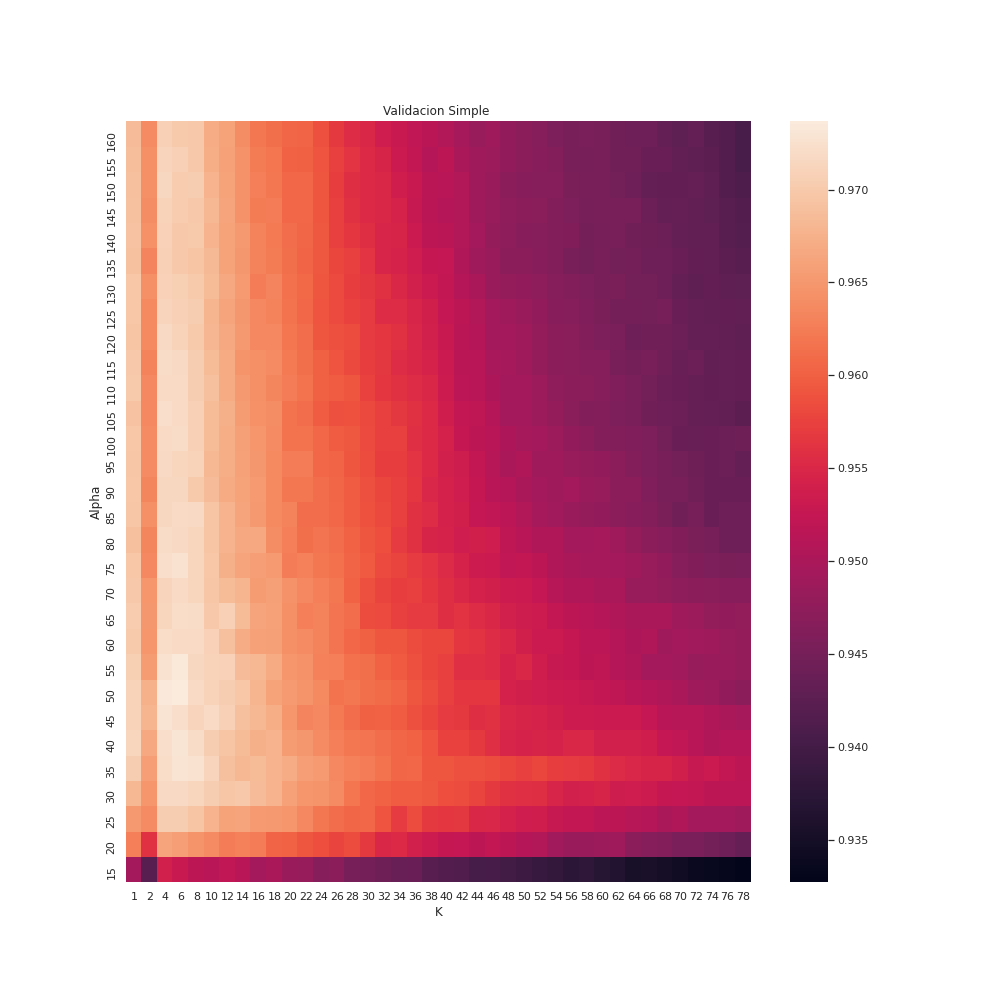
\includegraphics[width=12cm]{../images/validacionSimple_datasetCompleto_knnpca_k80}%
    \qquad
    \caption{Validacion Simple de kNN+PCA sobre el data-set completo}
    \label{knnpca_preliminar}%
\end{figure}


\begin{table}[h!]
    \begin{center}
        \begin{tabular}{|c|c|c|c|}
        \hline
        \textbf{$k$} & \textbf{$\alpha$} & \textbf{accuracy} \\
        \hline
        50 & 6 & 0.9736\\
        50 & 4 & 0.9734\\
        55 & 6 & 0.9733\\
        40 & 6 & 0.9739\\
        35 & 6 & 0.9728\\
        45 & 4 & 0.9728\\
        35 & 8 & 0.9726\\
        75 & 6 & 0.9726\\
        55 & 4 & 0.9726\\
        45 & 6 & 0.9723\\
        
        \hline
        \end{tabular}
        \caption{Accuracy de las mejores 10 parejas extraido de la Validacion Simple sobre el dataset completo para kNN+PCA.}
        \label{knnpca_valSimple_table}
    \end{center}
\end{table}

\subsection{Validación Cruzada}

Por último para conseguir el mejor parámetro o la mejor pareja en el caso de knn+pca se somete a los resultados previos a una corrida de validación cruzada ,con diez particiones, para evitar cualquier tipo de sesgo que pudiera tener nuestra anterior split de entrenamiento y validacion. 
El funcionamiento de la validación cruzada junto a la eleccion de su parámetros como diez se detalla en la seccion @LUIS.

\subsubsection{kNN}


$ k \in \{1,3,4,5,6,7,8,9,10,11\}$

\begin{table}[h!]
    \begin{center}
        \begin{tabular}{|c|c|}
        \hline
        \textbf{$k$} & \textbf{accuracy} \\
        \hline
        3 &  0.9671\\
        5 & 0.9668\\
        4 & 0.9664\\
        6 & 0.9656\\
        1 &  0.9654\\
        7 & 0.9653\\
        8 & 0.9640\\
        9 & 0.9633\\
        10 & 0.9629\\
        11 & 0.9623\\
        
        \hline
        \end{tabular}
        \caption{Accuracy promedio resultante de la Validacion Cruzada para kNN.}
        \label{knn_crossVal_table}
    \end{center}
\end{table}

\subsubsection{kNN+PCA}

En el caso de kNN+PCA  no solo tomamos las diez mejores parejas resultantes de la validación simple si no que extraemos los alpha, k de ellas y sometemos a validación cruzada a la combinacion de todos ellos parámetros.

$ k \in \{4,6,8\}$
\par
$alpha \in \{  35, 40, 45, 50, 55, 75 \}$
\begin{table}[h!]
    \begin{center}
        \begin{tabular}{|c|c|c|c|}
        \hline
        \textbf{$k$} & \textbf{$\alpha$} & \textbf{accuracy} \\
        \hline
        40 & 4 & 0.9716\\
        35 & 6 & 0.9713\\
        40 & 6 & 0.9712\\
        35 & 4 & 0.9712\\
        45 & 6 & 0.9711\\
        45 & 4 & 0.9711\\
        50 & 4 & 0.9710\\
        40 & 8 & 0.9710\\
        35 & 8 & 0.9710\\
        55 & 6 & 0.9708\\
        
        \hline
        \end{tabular}
        \caption{Accuracy de las mejores 10 parejas del total de 18 parejas extraido de la Validacion Cruzada .}
        \label{knnpca_crossVal_table}

    \end{center}
\end{table}

\subsection{ Testing sobre la mejor pareja : }


Utilizamos el 20$\%$ del data-set previamente separado para testear conseguir el $Accuracy$ de la mejor pareja.

\subsubsection{kNN}

$Accuracy_{mejor pareja} = 0.9661 $
\par
\vspace{0.5cm}
Aclaracion : la matriz de confusión se le reemplazaron los elementos de su diagonal por ceros para que sea más sencillo visualizar las demás casillas.
\begin{figure}[H]
    \centering
    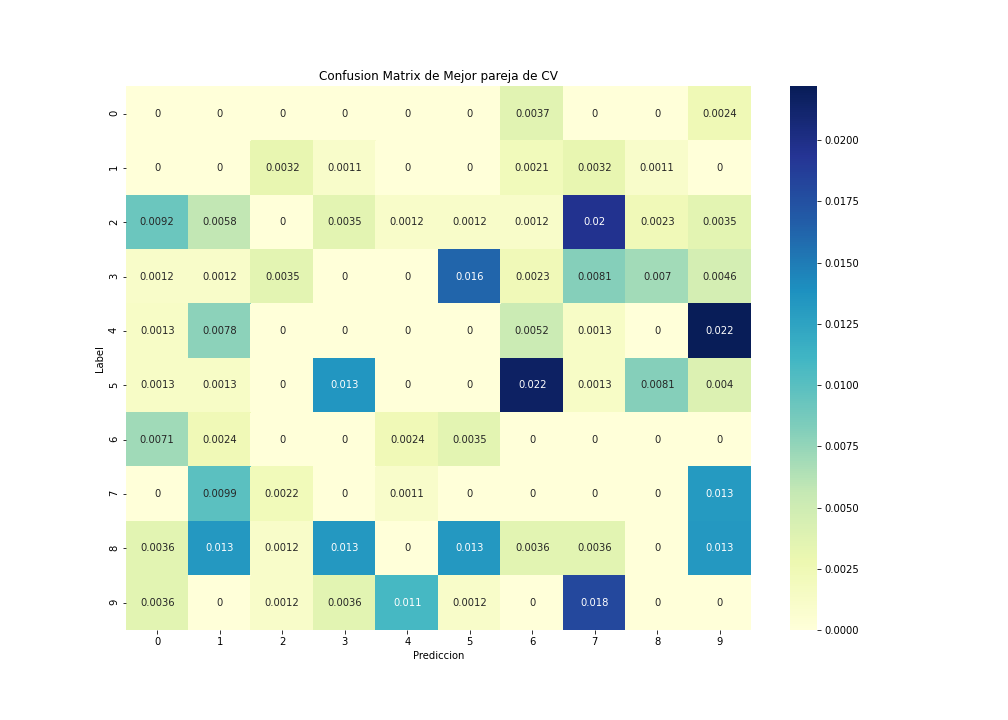
\includegraphics[width=14cm]{../images/../images/ConfMatrix_knn.png}%
    \qquad
    \caption{Matriz de Confusión para el mejor parámetro de kNN }
    \label{knn_MatrizConf}%
\end{figure}



\begin{figure}[H]
\begin{subfigure}{0.5\textwidth}
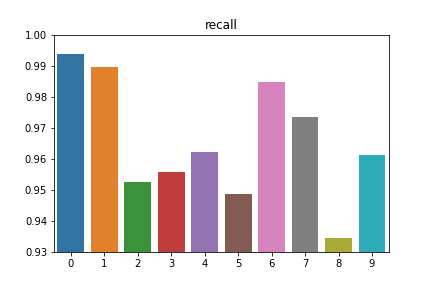
\includegraphics[width=0.9\linewidth, height=5cm]{../images/recall_knn.png} 
\caption{Recall del mejor parámetro}
\end{subfigure}
\begin{subfigure}{0.5\textwidth}
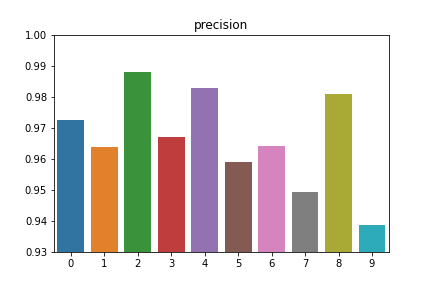
\includegraphics[width=0.9\linewidth, height=5cm]{../images/precision_knn.png} 
\caption{Precision del mejor parámetro}
\end{subfigure}
\caption{Metricas del mejor parametos para kNN.}
\label{knn_metricas}%
\end{figure}





\subsubsection{kNN+PCA}


\vspace{0.5cm}
$Accuracy_{mejor pareja} = 0.9725 $
\par
\vspace{0.5cm}
Aclaracion : la matriz de confusión se le reemplazaron los elementos de su diagonal por ceros para que sea más sencillo visualizar las demás casillas.
\begin{figure}[H]
    \centering
    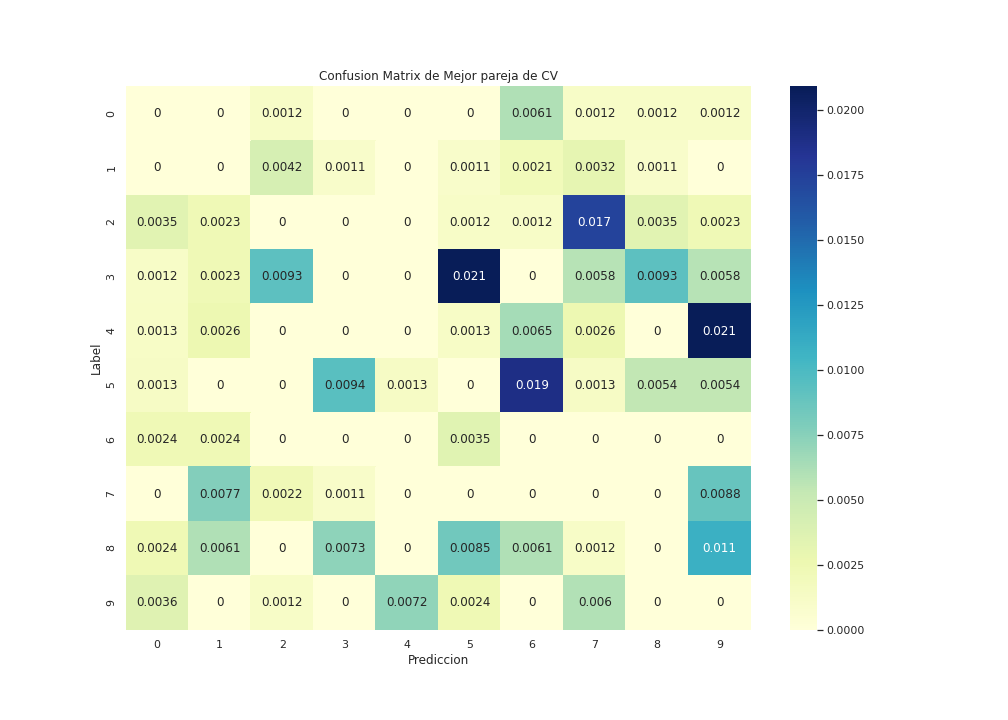
\includegraphics[width=14cm]{../images/../images/ConfMatrix_knnpca.png}%
    \qquad
    \caption{Matriz de Confusión para el mejor parámetro de kNN }
    \label{knnpca_MatrizConf}%
\end{figure}

\begin{figure}[h]
\begin{subfigure}{0.5\textwidth}
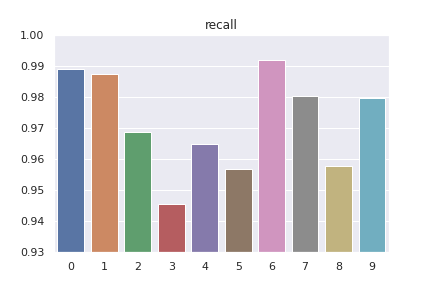
\includegraphics[width=0.9\linewidth, height=5cm]{../images/recall_knnpca.png} 
\caption{Recall de la mejor pareja}
\label{fig:metpca1}
\end{subfigure}
\begin{subfigure}{0.5\textwidth}
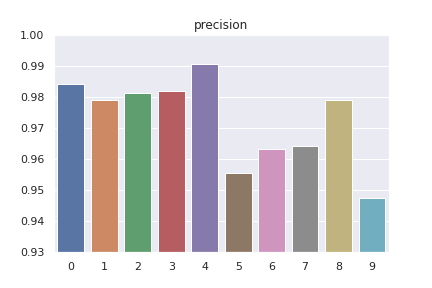
\includegraphics[width=0.9\linewidth, height=5cm]{../images/precision_knnpca.png} 
\caption{Precision de la mejor pareja}
\label{fig:metpca2}
\end{subfigure}
\caption{Metricas de la mejor pareja para kNN+PCA.}
\label{knnpca_metricas}%
\end{figure}


\subsection{Conclusión de los parámetros óptimos}


Como se puede observar tanto en las métricas y matriz de confusión de kNN como kNN+PCA para algunos dígitos estos métodos funcionan casi perfectamente (es el caso del uno y el cero), pero para otros como el tres por ejemplo su rendimiento decrece. Estas disparidades en la predicción hacen que nos planteamos algunas dudas , si estos datos mal clasificados pueden considerarse como outliers dado a q su morfología no se asemeja al dígito que dice su etiqueta o tal vez debemos modificar nuestro entrenamiento para llegar a mejorar la predicción de una clase complicado , si esto es asi tal vez se deba dejar de lado el accuracy general.
%al vez el 
%como por ejemplo tal vez con alguna elección de  parámetros en las que baje un poco el accuracy general podriamos lograr un desempeño mejor en algunos de estos dígitos complicados, otra posibilidad sería que necesitamos más datos de esos dígitos para entrenar el método y asi balancear el rendimiento de todas las clases.


\subsection{Análisis de datos malclasificados por nuestro mejor predictor}

\end{document}

\FloatBarrier
\newpage
\subsection{Tamaño del conjunto de entrenamiento}
En la sección anterior arribamos a la conclusión de cuáles son los intervalos óptimos para los parámetros de cada una de las técnicas. Más aún, escogimos los exponentes de estos rangos; aquellos valores de \emph{k} para \emph{kNN} y de $\alpha$ para \emph{PCA} que maximizan alguna de las métricas; en nuestro caso particular, fijamos la atención en el \emph{accuracy}. 
\par
Ahora bien, esta elección se basa en los resultados y el análisis de un experimento llevado a cabo sobre un conjunto de datos de un tamaño determinado. Entonces, surge la necesidad de corroborar la calidad óptima de estos valores al ser utilizados con conjuntos de entrenamiento de otras dimensiones. Es de interés observar si se produce un corrimiento de los intervalos previamente encontrados; o bien, si los exponentes de éstos continúan maximizando el \emph{accuracy}. 
\par
Con el fin de encontrar una respuesta a estas intrigas, planteamos una generalización del experimento hecho en la sección previa; variando -además- la cantidad de elementos que constituyen al conjunto de entrenamiento. Adicionalmente, ampliamos los rangos de los argumentos de las técnicas sobre los cuales experimentamos, para poder observar posibles movimientos de los intervalos óptimos. Nuevamente, para que la evaluación de las predicciones resulte más robusta se realizó validación cruzada con 10 \emph{folds}.
\par
A partir de los resultados obtenidos pudimos identificar tres dimensiones para analizar. En primer lugar, estudiamos el comportamiento de los valores óptimos para los parámetros de cada técnica a medida que varía el tamaño del conjunto de entrenamiento; lo que originalmente motivó a hacer el experimento. Luego, la relación entre la calidad de las predicciones y las dimensiones del conjunto; y finalmente, el costo temporal en relación a éste. En las siguientes secciones discutimos cada uno de estos aspectos con mayor detalle.
\subsubsection{Argumentos óptimos}
Retomamos la motivación original de esta sección: observar si los valores óptimos previamente encontrados dependen del tamaño del conjunto con el cual se entrena al predictor. Hay un especial interés en responder las siguientes preguntas: aquellos argumentos que maximizan el \emph{accuracy} para el conjunto utilizado en la sección anterior, ¿continuarán maximizando las métricas? En caso de no ser así, ¿seguirán siendo efectivos? A pesar de que se pueda perder calidad en los resultados, ¿podremos usarlos independientemente de la cantidad de datos de entrenamiento?
\par
[gráficos accuracy y precision en funcion k knn]
\par
Las figuras x-y muestran los resultados obtenidos para el caso donde se utiliza \emph{kNN} de manera individual. Cada una expone las métricas de \emph{accuracy} y \emph{precision} en función del parámetro \emph{k} para un conjunto de entrenamiento de tamaño determinado. A simple vista, notamos que ambas métricas presentan un comportamiento bastante similar; entonces, nos reducimos a discutir los resultados obtenidos desde el punto de vista del \emph{accuracy}. Luego, con la información expuesta podemos hacer dos observaciones principales. Por un lado, notamos que en todos los casos el intervalo óptimo para los valores de \emph{k} se posiciona entre los números $[1, 7]$. Esto nos da un indicio de que existe una suerte de relación independiente entre el tamaño del conjunto de entrenamiento y el rango óptimo de argumentos para \emph{kNN}. Por otro lado, vemos que conforme crece el tamaño del conjunto, el valor de \emph{k} que maximiza las métricas se va corriendo del 5 al 3. Particularmente, cuando el tamaño es 6000, el valor óptimo es 5; cuando éste es 12000, notamos una suerte de empate entre 3 y 5; y a partir de 18000, las métricas muestran mejores resultados con \emph{k} igual a 3. Con esto podemos dar una mínima garantía de que utilizar \emph{kNN} con un $k=3$ continúa siendo una elección adecuada independientemente de la cantidad de datos con la que se lo entrene. En la mayoría de los casos las mejores predicciones se encuentran asociadas a este argumento. Notemos, que el el caso particular donde el argumento óptimo resultó ser $k=5$, la diferencia entre las métricas para 3 y 5 no es del todo significativa. No obstante, esto último va a terminar dependiendo del área de aplicación. Finalemnte, esto deja la siguiente intriga: ¿qué ocurre cuando \emph{k} vale 4? Recordemos que experimentamos únicamente con los valores impares del intervalo $[1,15]$. Quizás, deberíamos reiterar el experimento con el intervalo $[1,7]$ y aumentar la granularidad.
\par
[heatmaps accracy segun k,alfa]
\par
Luego, en las figuras x-y se presentan la evaluación de los resultados obtenidos al combinar \emph{PCA} con \emph{kNN}. Como mencionamos en le párrafo anterior, escogimos exponer únicamente el caso del \emph{accuracy} debido a la semejanza en el comportamiento con las demás métricas. Estos mapas de calor muestran el \emph{accuracy} calculado para cada combinación de los parámetros \emph{k} y $\alpha$. Escogimos utilizar mapas de calor para poder observar qué forma tomaba el intervalo de parejas óptimas alrededor del mejor exponente. En primer lugar, observamos que los intervalos óptimos no se corrieron al variar el tamaño del conjunto de entrenamiento. Además, podemos ver que la pareja óptima converge a (\emph{k}=3, $\alpha=$35) conforme crece el tamaño. Concretamente, a partir de 18000, ya converge. Por lo tanto, podemos suponer que nuestra elección de pareja óptima también aplica para otros tamaños de \emph{trainset}; no necesariamente maximizará el \emph{accuracy} en todos los casos, pero si se mantendrá bastante cerca de la pareja en \emph{primer lugar}. Notemos que en la sección anterior se concluyó que esta era (4, 40). Sin embargo, cabe aclarar que en este experimento se decidió probar con los valores impares de los rangos, a diferencia del experimento previo, donde se prestó atención a los pares. De todas formas, vemos que (3,35) y (4,40) son parejas \emph{hermanas} si tenemos en cuenta el tema de paridad en conjunción con los incrementos de 10 unidades en el caso del $\alpha$. Aún así, surge la necesidad de experimentar con mayor granularidad en torno a estas parejas.
\par
Entonces, con el análisis en esta primera sección podemos aportar una mínima garantía al supuesto de relación independiente entre los argumentos óptimos de las técnicas y las dimensiones del conjunto de entrenamiento.
\subsubsection{Calidad de las predicciones}
En esta sección hacemos un pequeño análisis de la calidad de los resultados generados por cada técnica a medida que varía el tamaño del conjunto de entrenamiento. En primer lugar, estudiamos el comportamiento de algunas métricas para cada técnica por separado. Luego, las comparamos entre sí. Se intentan responder preguntas como: ¿Cómo se relacionan la técnicas con el tamaño del conjunto de entrenamiento? ¿Podemos jerarquizar las técnicas? ¿Habrá tamaños para los cuales una es más adecuada que la otra?
\par
Teniendo en cuenta el análisis de la sección [sección argumentos óptimos], decidimos estudiar únicamente los resultados generados por los argumentos que maximizan las métricas. Particularmente $k=3$ y $\alpha=35$.
\par
[grafico comparacion métricas]
\par 
La figura x expone la evaluación de los resultados obtenidos por cada técnica en relación a la cantidad de datos con la cual se entrenó. Podemos observar que para las técnicas la relación entre la calidad de las predicciones y el tamaño del conjunto de entrenamiento es proporcional. Además notamos que el crecimiento en función del tamaño es similar en ambos casos. Creemos que la razón de esto radica en que conforme crece la cantidad de datos de entrenamiento se tienen más instancias de cada clase; particularmente, de la clase relevante a una predicción determinada. Luego, cuando se busquen los $k$ vecinos más cercanos a la entrada, habrá una mayor probabilidad de que las instancias parecidas a la entrada que pertenezcan a la clase relevante. Ahora bien, esto se cumple bajo el supuesto de que conforme crece el conjunto de entrenamiento se mantiene un cierto balance entre las distintas clases y que la mayoría de las instancias se encuentra bien definida. Por otro lado, vemos que la relación entre calidad y tamaño del conjunto no es necesariamente lineal: a partir del 18000 el crecimiento resulta ser menos drástico.
\par
Si bien presentan una curva de crecimiento similar, notamos una clara diferencia entre los valores concretos de cada técnica. Para todos los conjuntos de entrenamiento hay una diferencia de aproximadamente 0,1 entre los valores de \emph{accuracy} de cada una; en todos los casos, se favorece a la combinación de \emph{PCA} y \emph{kNN}. Entonces, pareciera ser que la utilización de \emph{PCA} para reducir redundancias entre los datos del conjunto de entrenamiento y maximizar la varianza de éstos tiene como efecto que las predicciones realizadas con \emph{kNN} resulten más acertadas en el caso general. Más aún, destacamos la posibilidad de que esta mejora en la calidad de los resultados se mantenga constante independiente de la cantidad de datos con la que se entrena.
\par
Cerrando esta sección, concluimos que la calidad de las predicciones aumenta a la par con el tamaño del conjunto de entrenamiento; y que el crecimiento observable es similar en ambos casos. Luego, notamos una clara mejora al combinar \emph{PCA} con \emph{kNN}.
\subsubsection{Costo temporal}
Habiendo establecido que aplicar \emph{PCA} sobre los datos antes de predecir con \emph{kNN} genera resultados de mayor calidad, surge la necesidad de estudiar el costo temporal asociado a la presencia o a la ausencia de \emph{PCA}. A simple no podemos observar una jerarquía muy obvia. En ambos casos hay motivos para creer que una será consumira menos tiempo que la otra. Por un lado, tenemos que el uso de \emph{PCA} implica la neceisadad de calcular una serie de autovector y autovalores, lo cual -aplicando el metodo de la potencia- podría implicar un costo adicional no trivial. Por el otro lado, tenemos que los datos resultantes de haberles aplicado la transformación asociada son de menor dimensión.Esto podría implicar una reducción en el timpo de ejecución de \emph{kNN}; notamos la relación directa entre las dimensiones del conjunto de entrenamiento y el costo temporal de buscar los vecinos más cercanos.
\par
Con los tiempos obtenidos de cronometrar las distintas corridas del experimento construimos las figuras x e y. La figura x muestra únicamente los tiempos de ejecución asociados a la función de predicción de las dos variantes; mientras que en la figura y se incluye el costo asociado a aplicar la técnica \emp{PCA}. Curiosamente, notamos que en ambos casos la diferencia entre los costos temporales se va haciendo cada vez más significativa conforme aumenta el tamaño del \emph{set} de entrenamiento. La reducción en la dimensión pareciera ser un factor de gran importancia para el tiempo de ejecución. Además, vemos que los cálculos asociados a \emp{PCA} no demuestran ser lo suficientemente altos como para generar una suerte de \emp{trade-off} entre la calidad de los resultados y el costo temporal. El único caso donde supera a la versión individual de \emp{kNN} es cuando el tamaño del \emp{trainset} es muy pequeño. Sin embarge, conforme aumenta la cantidad de datos de entrenamiento, el costo asociado a las predicciones luego de haber utilizado \emph{PCA} no crece de manera drástica; en contraposición a la otra versión.
\par
En suma, podemos concluir que la combinación de \emp{PCA} con \emp{kNN} representa una mejora no trivial tanto en la calidad de las predicciones como en el costo temporal de la técnica. 

\FloatBarrier
\newpage
\subsection{Balanceo y morfología}
La intención de esta sección es ver tanto cómo se comporta el OCR al contar con una base de datos de entrenamiento totalmente balanceada y desbalanceada como la morfología de los dígitos y qué consecuencias pueden traer. Como tal no realizaremos iteraciones sobre el alpha o el k, asumiendo valores fijos iguales a los ``mejores'' encontrados en las secciones anteriores.

En la tabla \ref{tab:totalDigitos} se puede ver la cantidad por digitos del dataset completo. Como el 5 (del que menos hay) tiene 3795 instancias, no podemos elegir más de esa cantidad. En todos los experimentos que siguen vamos a utilizar 3795 instancias, 2277 de entrenamiento y 1518 de validación.

\begin{table}[h]
\centering
\begin{tabular}{|c|c|}
\hline
0 & 4132 \\ \hline
1 & 4684 \\ \hline
2 & 4177 \\ \hline
3 & 4351 \\ \hline
4 & 4072 \\ \hline
5 & 3795 \\ \hline
6 & 4137 \\ \hline
7 & 4401 \\ \hline
8 & 4063 \\ \hline
9 & 4188 \\ \hline
\end{tabular}
\caption{Cantidad de instancias por dígito}
\label{tab:totalDigitos}
\end{table}

Primero vimos qué pasaba al tener un conjunto de entrenamiento totalmente balanceado. Como podemos ver en la fig.\ref{fig:bal_recall_prec} el sistema tiene bastante buena precisión y recall para cada una de las clases, con un accuracy de 0.925.
\begin{figure}[h]
    \centering
    \begin{subfigure}{.5\textwidth}
        \centering
        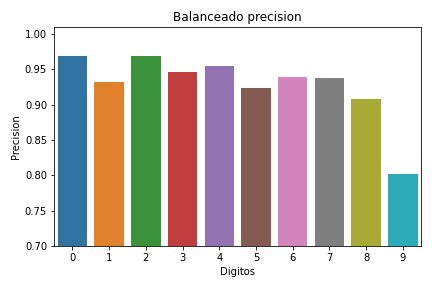
\includegraphics[width=.8\linewidth]{images/balanceo/Balanceado precision_3795.png}
    \end{subfigure}%
    \begin{subfigure}{.5\textwidth}
        \centering
        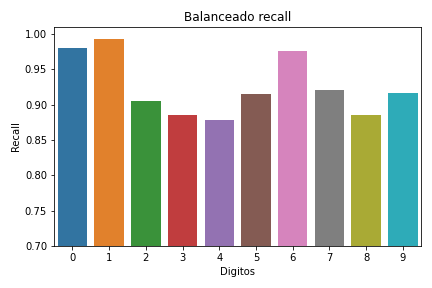
\includegraphics[width=.8\linewidth]{images/balanceo/Balanceado recall_3795.png}
    \end{subfigure}%
    \caption{Recall y precision de balanceado}
    \label{fig:bal_recall_prec}
\end{figure}

Como la precisión del 9 es la más baja intentamos mejorar esto agregando más instancias del mismo, cabe aclarar que cuando decimos agregar es en realidad un desbalance pero tenemos la misma cantidad de instancias de entrenamiento. La proporción normalizada de 9s es 0.16 y 0.093 para el resto. En la figura \ref{fig:9s_recall_prec} se ve que, contrario a lo que suponíamos, la precisión baja aún más y además empeora el recall de los 4s.
\begin{figure}[h]
    \centering
    \begin{subfigure}{.5\textwidth}
        \centering
        \includegraphics[width=.8\linewidth]{images/balanceo/Con más 9s precision_3795.png}
    \end{subfigure}%
    \begin{subfigure}{.5\textwidth}
        \centering
        \includegraphics[width=.8\linewidth]{images/balanceo/Con más 9s recall_3795.png}
    \end{subfigure}%
    \caption{Recall y precision de desbalance con más 9s}
    \label{fig:9s_recall_prec}
\end{figure}

\FloatBarrier
Pero si esto es así entonces \textit{¿Qué pasa si agregamos más 4s en vez de 9s?}. Al hacer el intento, con proporción normalizada de 0.16 para los 4s y 0.093 para el resto, vimos que mejora el recall para el 4 sin bajar tanto el del 9 y obtiene mejor accuracy general, esto se puede ver en la figura \ref{fig:4s_recall_prec}.
\begin{figure}[h]
    \centering
    \begin{subfigure}{.5\textwidth}
        \centering
        \includegraphics[width=.8\linewidth]{images/balanceo/Con más 4s precision_3795.png}
    \end{subfigure}%
    \begin{subfigure}{.5\textwidth}
        \centering
        \includegraphics[width=.8\linewidth]{images/balanceo/Con más 4s recall_3795.png}
    \end{subfigure}%
    \caption{Recall y precision de desbalance con más 9s}
    \label{fig:4s_recall_prec}
\end{figure}

\FloatBarrier
Esto tiene sentido, ya que el mayor error está cuando los valores son 4s pero clasifica erroneamente como 9, como se puede ver en \ref{fig:bal_conf}. Por ende al tener más instancias de 4s le estamos dando al sistema más vecinos para comparar del valor con el que más flaquea, esto aumenta el recall del 4 al dar menos falsos negativos, luego como el valor predecido era 9 la precisión de este último aumenta ya que hay menos falsos positivos.
\begin{figure}[h]
 \centering
 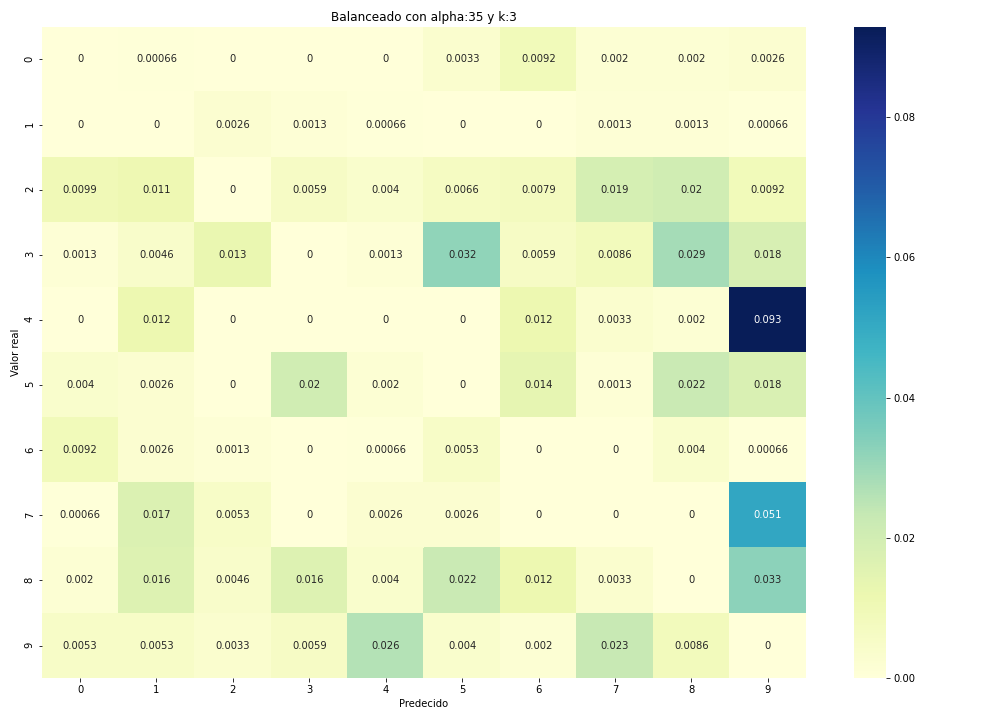
\includegraphics[width=0.8\linewidth]{images/balanceo/Balanceado con alpha:35 y k:3_3795.png}
 \caption{Matriz de confusión para dataset balanceado (diagonal anulada)}
 \label{fig:bal_conf}
\end{figure}

A modo de resúmen y para facilitar su comparación, en la figura \ref{fig:comparaciones} se puede ver la precisión, recall y f1 para cada una de las clases y cada uno de los desbalances propuestos hasta ahora.
\begin{figure}
    \centering
    \subfloat{{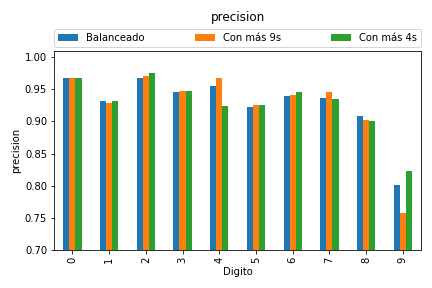
\includegraphics[width=.5\linewidth]{images/balanceo/primeros3exp_precision_3795.png} }}%
    
    \subfloat{{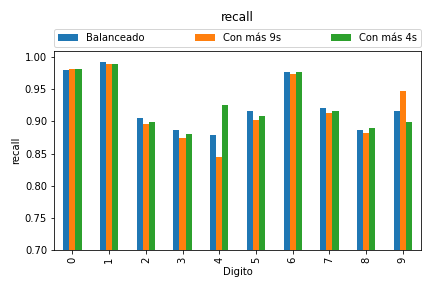
\includegraphics[width=.5\linewidth]{images/balanceo/primeros3exp_recall_3795.png} }}%
    \subfloat{{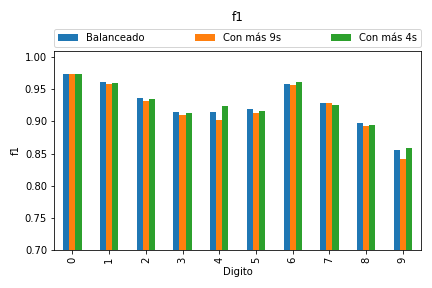
\includegraphics[width=.5\linewidth]{images/balanceo/primeros3exp_f1_3795.png} }}%
    
    \caption{Precisión, recall y f1 por clase para los primeros tres desbalances}
    \label{fig:comparaciones}
\end{figure}

\FloatBarrier

Creemos que los errores se deben a la morfología de estos números, ya que basta redondear un poco la línea del cuatro para que se confundan. De hecho, mirando a mano algunas de las imágenes (fig.\ref{fig:ejemplos_feos}) con las cuáles comete errores podemos ver casos polémicos; algunos no tienen la mejor de las calidades o están girados, otros directamente fueron mal catalogados. Cabe destacar que la última fija son dígitos manuscritos ingresados por nosotros, utilizando nuestra herramienta \textit{Coso Recognizer}\footnote{El nombre fue una joda y quedó, disculpas} la cuál se puede usar corriendo el script de mismo nombre\footnote{Está en la carpeta notebooks, requiere tkinter (apt-get install python3-tk)}.
\begin{figure}[h]
    \centering
    \subfloat{{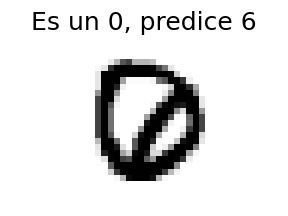
\includegraphics[width=.18\linewidth]{images/balanceo/digitosFeos/es0_pred6_4.png} }}%
    \subfloat{{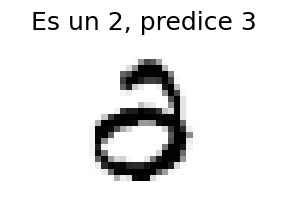
\includegraphics[width=.18\linewidth]{images/balanceo/digitosFeos/es2_pred3_1.png} }}%
    \subfloat{{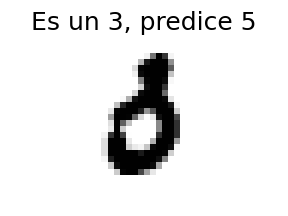
\includegraphics[width=.18\linewidth]{images/balanceo/digitosFeos/es3_pred5_9.png} }}%
    \subfloat{{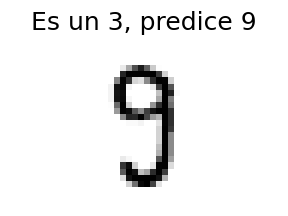
\includegraphics[width=.18\linewidth]{images/balanceo/digitosFeos/es3_pred9_3.png} }}%
    
    \subfloat{{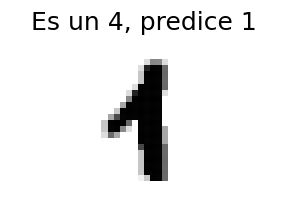
\includegraphics[width=.18\linewidth]{images/balanceo/digitosFeos/es4_pred1_1.png} }}%
    \subfloat{{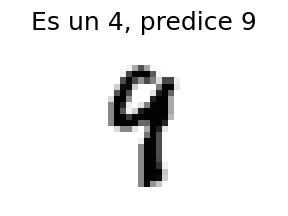
\includegraphics[width=.18\linewidth]{images/balanceo/digitosFeos/es4_pred9_9.png} }}%
    \subfloat{{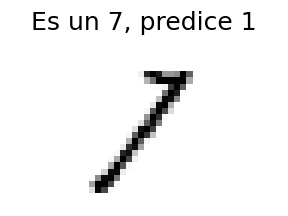
\includegraphics[width=.18\linewidth]{images/balanceo/digitosFeos/es7_pred1_0.png} }}%
    \subfloat{{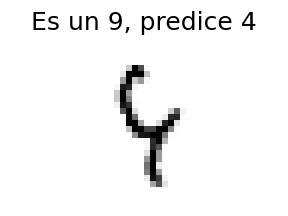
\includegraphics[width=.18\linewidth]{images/balanceo/digitosFeos/es9_pred4_0.png} }}%
    
    \subfloat{{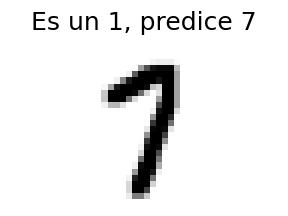
\includegraphics[width=.18\linewidth]{images/balanceo/digitosFeos/aMano_es1_pred7.png} }}%
    \subfloat{{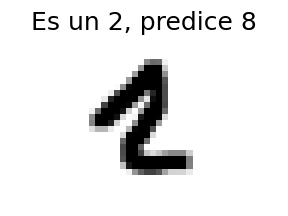
\includegraphics[width=.18\linewidth]{images/balanceo/digitosFeos/aMano_es2_pred8.png} }}%
    \subfloat{{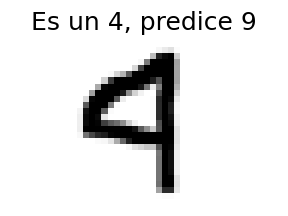
\includegraphics[width=.18\linewidth]{images/balanceo/digitosFeos/aMano_es4_pred9.png} }}%
    \subfloat{{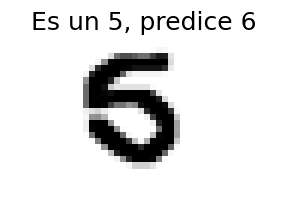
\includegraphics[width=.18\linewidth]{images/balanceo/digitosFeos/aMano_es5_pred6.png} }}%
    
    \caption{Casos horriblemente particulares}
    \label{fig:ejemplos_feos}
\end{figure}

\FloatBarrier
Hasta ahora sabemos que el desbalance no es inherentemente malo sino que podría beneficiarnos, entonces surge la pregunta \textit{¿Cuál es la configuración (proporciones de dígitos) que más accuracy genera?}

Para empeza desbalanceamos a mano utilizando como guía el recall de cada clase, en favor de los que menos poseen. Probamos con las proporciones: 

\begin{description}
 \item [Muchos 4s, más 3s] proporción de 0.11, 0.18 para el 3 y 4 (resp.) y 0.093 para el resto. 
 \item [Muchos 4s, más 3s, 7s y 8s] proporción de 0.18 para el 4, 0.11 para el 3,7 y 8 y 0.087 para el resto. 
\end{description}

En la figura \ref{fig:acc} se ve que con más 4s y 3s se obtiene aún más accuracy pero ya al desbalancear 7s y 8s volvemos a perder exactitud, aunque aún es mejor que el set balanceado.
\begin{figure}[h]
 \centering
 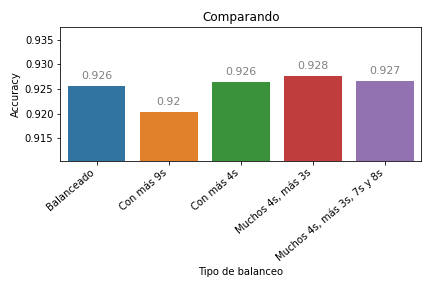
\includegraphics[width=0.65\linewidth]{images/balanceo/acc.png}
 \caption{Accuracy para cada uno de los casos.}
 \label{fig:acc}
\end{figure}
 
\FloatBarrier
Luego generamos automáticamente algunas variaciones de proporciones en función de encontrar alguno con mayor accuracy. Dividimos los dígitos en dos grupos, los del primero tienen una proporción fija y los restantes se dividen lo que queda equitativamente. Variamos la proporción fija en [0.11, 0.18, 0.19] y como grupos se tomaron todas las combinaciones de 1 y 2 elementos. Estos casos no llegaron a ser tan buenos como \textit{Muchos 4s, más 3s}, en la figura \ref{fig:accAutom} se puede ver la variación de los accuracy conseguidos.

\begin{figure}[h]
 \centering
 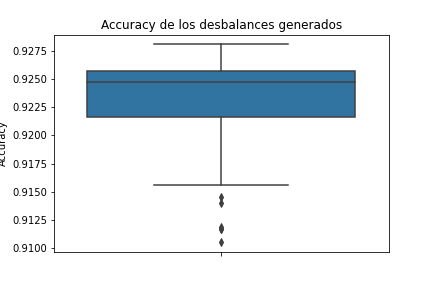
\includegraphics[width=0.65\linewidth]{images/balanceo/acc_generados.png}
 \caption{Accuracy casos generados}
 \label{fig:accAutom}
\end{figure}

\FloatBarrier


\FloatBarrier
\newpage
\subsection{Sobre Cross Validation con K-Fold}

Como fue propuesto por la cátedra, para validar que la elección de nuestros parámetros para el sistema lleven luego a una buena generalización al momento de clasificar dígitos, utilizamos la técnica de cross validation con K-Fold.

Brevemente, para el caso de KNN+PCA, por ejemplo, tenemos que elegir entre $(k_i, \alpha_i)$ óptimos, por lo que para cada par se partirá el trainset disponible en $K$ conjuntos para luego hacer $K$ pruebas, donde en cada una de ellas la unión de $K-1$ conjuntos pasan a ser un nuevo trainset y el restante pasa a ser un nuevo testset. Al menos cada conjunto fue un testset después de haber aplicado K-Fold. Luego, promediando algúna métrica de performance entre las $K$ disponibles se puede obtener el valor final para la misma, la cual puede ser comparada después con las generadas por otros pares de parámetros. Los elegidos van a poder ser validados con el testset original.

Las preguntas que se listan a continuación surgieron de pensar las cosas mencionadas en el párrafo anterior y se realizaron pruebas teniendo en cuenta los siguientes atributos:

\begin{itemize}
    \item \textbf{Métrica de performance}: Accuracy, tomando la media.
    \item \textbf{Algoritmo}: KNN+PCA
    \item \textbf{Rango de $K$}: $\{5, 10, 15, 20\}$
    \item \textbf{Rango de $k$}: $\{1\dots53, 2\}$
    \item \textbf{Rango de $\alpha$}: $\{10\dots120, 10\}$
    \item \textbf{Dataset}: Primeros 10000 elementos del dataset original, tomando el $80\%$ como trainset y el restante como testset.
\end{itemize}

\subsubsection{¿Qué valor debería tener K?}\label{KFoldValueK}

Elegir los parámetros con validación simple consiste en hacer $n$ corridas de nuestro sistema, donde $n$ es el número de parámetros candidatos que tenemos. Hacerlo con cross validation utilizando K-Fold nos lleva a realizar $n * K$ corridas del sistema, por lo que el tiempo de duración del experimento puede llegar a ser grande. Dependiendo de, entre otras cosas, el tamaño del dataset y la eficiencia general de los algoritmos.

Esto nos llevó a probar inicialmente con una serie de valores fijos para $K$ y una parte del dataset original para ver si, la métrica de performance variaba mucho, e inferir en ese caso si vale el costo temporal o no hacer la validación con valores de $K$ cada vez más altos.

\begin{itemize}
    \item \textbf{Pregunta}: ¿Será apreciable la variación de nuestra métrica de performance si K crece?
    \item \textbf{Hipótesis}: Si: incrementar $K$ permitiría ver como se comporta el sistema con $K$ trainsets distintos, por lo que es factible que mientras más trainsets existan, se van a poder elegir parámetros que generalicen mejor y maximicen la métrica de performance.
\end{itemize}

\subsubsection*{Análisis y resultado}

Para uno de los pares estudiados $(k = 3, \alpha = 40)$

\begin{figure}[H]
    \centering
    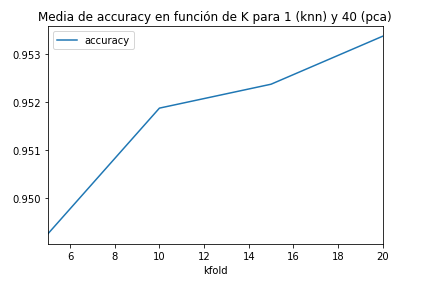
\includegraphics[scale=0.7]{images/KFoldIncreasingK.png}
    \caption{Variación del accuracy en función de $K$ para uno de los pares estudiados.}
    \label{fig:KFoldIncreasingK}
\end{figure}

Como se puede apreciar en la figura \ref{fig:KFoldIncreasingK}, efectivamente, hubo un incremento en el accuracy.

A juzgar por esta prueba, mientras mayor sea $K$, mayor es el accuracy por lo que parece conveniente, al menos tomar $K = 20$.

¿Pero que sucede si tomamos $K$ arbitrariamente grande? Podríamos decir con cierta seguridad que el sistema se encontraría overfitteado, lo que nos llevaría a tener predicciones pobres al validar.

Elegir $K$ arbitraríamente alto tampoco seria productivo.

\subsubsection{¿Qué relación hay entre K y el tamaño del trainset?}\label{KFoldTrainSizeAcc}

Para la siguiente prueba, el trainset definido de 8000 elementos, lo particionamos en cuatro trainsets: el primero de 2000, el segundo de 4000, el tercero de 6000 y el último (el completo) de 8000 elementos.

\begin{itemize}
    \item \textbf{Pregunta}: A mayor tamaño del trainset y de $K$, ¿el accuracy también será mayor?
    \item \textbf{Hipótesis}: Si: de alguna forma será mayor en proporción a la cantidad de elementos que haya en el conjunto de entrenamiento. De esta forma, la mejor elección de nuestros parámetros la vamos a poder realizar con el dataset completo (42000 elementos, 33600 para el trainset) propuesto por la cátedra.
\end{itemize}

\subsubsection*{Análisis y resultado}

La evaluación fue consistente con la hipótesis planteada, observando el par mencionado con anterioridad.

\begin{figure}[H]
    \centering
    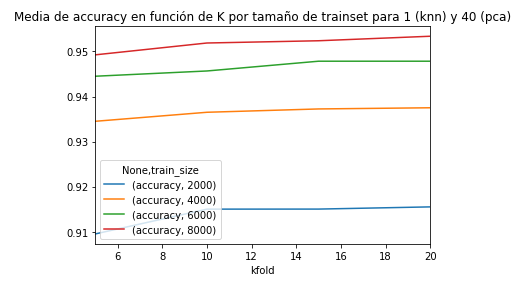
\includegraphics[scale=0.7]{images/KFoldAccTrainSize.png}
    \caption{Accuracy vs K: La mayor diferencia parece lograrse no variando K, si no variando el tamaño del trainset.}
    \label{fig:KFoldAccTrainSize}
\end{figure}

En la figura \ref{fig:KFoldAccTrainSize} se puede observar, análogamente al caso anterior que para diferentes tamaños de trainset se ven pequeñas mejoras a medida que aumenta el valor de $K$, pero la diferencia notable en el accuracy está precisamente en el tamaño de mencionado conjunto. Aunque también es llamativo ver que la diferencia de la métrica entre el conjunto de 4000 y el de 2000 elementos es mayor a la que hay entre el conjunto de 6000 y 4000 elementos, y a su vez esta es mayor a la diferencia entre el conjunto de 8000 y el de 6000 elementos, lo que nos lleva a pensar que hay un límite para la mejora por el tamaño del trainset y que entrenar nuestro sistema con el dataset completo (42000 * 0.8) puede dejar esta métrica cercano a él.

\subsubsection{¿Conviene utilizar K-Fold? ¿Cuándo no?}

Utilizar K-Fold nos resulta útil para elegir los parámetros con cierta confianza de que no van a haber mayores problemas generalizando a datos desconocidos. A cambio permitimos que la información se reorganice en cada prueba de diferentes maneras. Eso mismo puede ser prohibitivo para modelos en los que haya una componente temporal presente, dado que se pierde el sentido en la información.

\subsubsection{Finalmente: ¿qué valor debería tener K?}

Vimos en la subsección \ref{KFoldValueK} que podriamos tomar $K=20$, dado que a mayor $K$, mayor accuracy. Pero también comentamos que el aumento no parecia ser significativo para el tiempo demorado.

En \ref{KFoldTrainSizeAcc} vimos que la mayor confianza se obtiene cuando el trainset tiene un tamaño grande. Esto tiene sentido dado que se entrena el sistema con más variaciones de las que se disponen con $K$ más chicos.

De los resultados obtenidos, para la configuración de la prueba mencionada previamente, las mostraron mayor accuracy fueron:

\begin{table}[h!]
    \begin{center}
        \begin{tabular}{|c|c|c|c|}
        \hline
        \textbf{$K$} & \textbf{$k$} & \textbf{$\alpha$} & \textbf{accuracy medio} \\
        \hline
        5 & 3 & 40 & 0.95\\
        10 & 3 & 40 & 0.9507\\
        15 & 3 & 40 & 0.9516\\
        20 & 5 & 50 & 0.9522\\
        \hline
        \end{tabular}
        \caption{Accuracy medio más alto para distintas configuraciones de K-Fold.}
        \label{kfold_table_1}
    \end{center}
\end{table}

Obteniendo la configuración $(3, 40)$ un accuracy mayor a la que obtuvo el par $(5, 50)$ en el testset final ($0.9645$ vs $0.9625$ respectivamente). Una elección razonable luego, sería tomar $K=15$ para hacer las pruebas. No obstante hay que tener presente que: esto es un ejemplo sobre una porción del dataset original, y el tiempo para calcular las pruebas con ese valor de $K$ puede ser significativo, por lo que finalmente $K=10$ es la elcción que tomamos para llevarlas acabo.
